\let\negmedspace\undefined
\let\negthickspace\undefined
%\RequirePackage{amsmath}
\documentclass[journal,12pt,onecolumn]{IEEEtran}
\usepackage{titlesec}
 \usepackage[utf8]{inputenc}
 \usepackage{graphicx}
 \usepackage{amsmath}
 \usepackage{mathrsfs}
\usepackage{txfonts}
\usepackage{stfloats}
\usepackage{bm}
\usepackage{cite}
\usepackage{cases}
\usepackage{subfig}
 \usepackage{amsfonts}
 \usepackage{amssymb}
 \usepackage{enumitem}
\usepackage{mathtools}
\usepackage{tikz}
\usepackage{circuitikz}
\usepackage{verbatim}
\usepackage[breaklinks=false,hidelinks]{hyperref}
\usepackage{listings}
\usepackage{calc}
\usepackage{float}
\usepackage{longtable}
\usepackage{multirow}
\usepackage{multicol}
\usepackage{color}
\usepackage{array}
\usepackage{hhline}
\usepackage{ifthen}
\usepackage{chngcntr}

\titleformat*{\section}{\color{teal}\LARGE\bfseries\filcenter}
\titleformat*{\subsection}{\color{blue}\large\bfseries}

\title{\color{teal} Warbler}
\author{Nunsavath Sree Harsha (CS21BTECH11042) \\ Rajiv Shailesh Chitale (CS21BTECH11051) \\ Vishal Vijay Devadiga (CS21BTECH11061)}

\begin{document}
\maketitle
\begin{center}
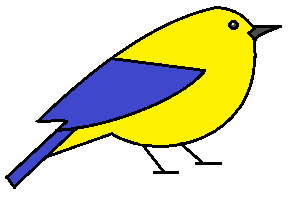
\includegraphics[width=0.3\linewidth]{logo.png}\\[1ex] 
\end{center}

\section*{\textbf{Description}}
Our project entails the creation of a social media platform called {\color{blue}Warbler}. It is inspired by Twitter.

\section*{\textbf{Tech Stack}}
\subsection*{\textbf{Front end}} HTML/CSS, JavaScript for an interactive UI
\subsection*{\textbf{Back end}} Java for more complicated algorithms and Object-Oriented Programming
\subsection*{\textbf{Database}} MySQL to store data persistently

\section*{\textbf{Features}} 
\subsection*{\textbf{Sign in / Sign up}}
\noindent A person over the minimum age of 13 can register on our platform with an unique username.
Once the person has registered, they will be able to login into the website.
%
\subsection*{\textbf{Profile}}
\noindent Each user has a customizable profile which includes:
\begin{itemize}
    \item Custom display name and display photo
    \item Bio containing short description of the user
    \item Details including date of birth, location and website
    \item Date of joining the platform
    \item Posts liked by the user
    \item Post history of the user
    \item List of followers
    \item List of users being followed
\end{itemize}
%
\subsection*{\textbf{Posts}}
Users can create posts and can also schedule it at a given time
A post can contain:
\begin{itemize}
    \item Text (upto 280 characters)
    \item Photos (upto 4 photos)
    \item Video (upto 140 seconds)
    \item Gif (upto 1 gif)
    \item Poll
    \item Content and spoiler warnings
    \item Tags and reply permissions
\end{itemize}
The following actions can be taken on a post:
\begin{itemize}
    \item Reply 
    \item Repost
    \item Like 
    \item Share
    \item Report
    \item Bookmark
\end{itemize}
%
\subsection*{\textbf{Direct messages}}
\begin{itemize}
    \item Accept or deny requests for direct messages
    \item These messages can also contain media
\end{itemize}
%
\subsection*{\textbf{Feed}}
\begin{itemize}
    \item Promoted posts
    \item Depending on popularity, and users under following
    \item Suggested to follow
    \item Mute users from feed
\end{itemize}
%
\subsection*{\textbf{Search}}
\begin{itemize}
    \item Search for posts and users
    \item Results based on hashtags 
\end{itemize}
%
\subsection*{\textbf{Settings}}
\begin{itemize}
    \item Change password
    \item Deactivate account
    \item Change font size
    \item Switch between dark and light mode
    \item Notification settings
\end{itemize}
\subsection*{\textbf{More}}
%
\begin{itemize}
    \item Block a user
    \item Admins can ban users having many reports
    \item Spam protection
    \item Notifications from replies, tags and likes.
\end{itemize}

\end{document}
